% latex table generated in R 3.6.3 by xtable 1.8-4 package
% Thu Jan 18 11:47:49 2024
\begin{table}[ht]
\centering
\begin{tabular}{rlrrr}
  \hline
 & OTU & MeanRA & MedianRA & SE \\ 
  \hline
419610 & Methylorubrum extorquens & 0.00006388 & 0.00005553 & 0.00001112 \\ 
  33995 & Komagataeibacter europaeu & 0.00003956 & 0.00003942 & 0.00000393 \\ 
  391595 & Roseobacter litoralis & 0.00004400 & 0.00004449 & 0.00000196 \\ 
  1795043 & Burkholderia sp. PAMC 2656 & 0.00005138 & 0.00004995 & 0.00000407 \\ 
  1267562 & Cupriavidus gilardii & 0.00005167 & 0.00003969 & 0.00001344 \\ 
  876364 & Cupriavidus sp. USMAA2- & 0.00002995 & 0.00002911 & 0.00000219 \\ 
  2771360 & Cupriavidus sp. ISTL & 0.00003866 & 0.00003090 & 0.00000863 \\ 
  2049589 & Pseudomonas sp. HLS- & 0.00005410 & 0.00004569 & 0.00000941 \\ 
  2320270 & Pseudomonas sp. DG56- & 0.00004612 & 0.00003992 & 0.00000702 \\ 
  1758730 & Pseudomonas sp. BIOMIG1BA & 0.00001259 & 0.00001161 & 0.00000142 \\ 
  658629 & Pseudomonas sessilinigene & 0.00001146 & 0.00000998 & 0.00000197 \\ 
  47883 & Pseudomonas synxanth & 0.00008678 & 0.00008019 & 0.00000943 \\ 
  46679 & Pseudomonas mucidolen & 0.00004223 & 0.00003787 & 0.00000416 \\ 
  384676 & Pseudomonas entomophila & 0.00008616 & 0.00007318 & 0.00001122 \\ 
  104087 & Pseudomonas frederiksbergensi & 0.00008741 & 0.00008464 & 0.00000976 \\ 
  364197 & Pseudomonas pohangensi & 0.00007947 & 0.00006237 & 0.00001242 \\ 
  1853130 & Pseudomonas silesiensi & 0.00004622 & 0.00004075 & 0.00000500 \\ 
  191390 & Pseudomonas palleronian & 0.00005105 & 0.00004380 & 0.00000627 \\ 
  158627 & Pseudomonas gramini & 0.00003343 & 0.00002934 & 0.00000424 \\ 
  471 & Acinetobacter calcoaceticu & 0.00000608 & 0.00000477 & 0.00000161 \\ 
  1134687 & Klebsiella michiganensi & 0.00003877 & 0.00004298 & 0.00000510 \\ 
  1646377 & Rouxiella badensi & 0.00003244 & 0.00003568 & 0.00000289 \\ 
  92644 & Streptomyces malaysiensi & 0.00003700 & 0.00004094 & 0.00000395 \\ 
  1935 & Streptomyces violaceorube & 0.00002474 & 0.00002450 & 0.00000171 \\ 
  145458 & Rathayibacter toxicu & 0.00003676 & 0.00003675 & 0.00000324 \\ 
  1933880 & Glutamicibacter halophytocol & 0.00006150 & 0.00005642 & 0.00000364 \\ 
  29311 & Mycobacterium haemophilu & 0.00007257 & 0.00006852 & 0.00000533 \\ 
  1833 & Rhodococcus erythropoli & 0.00004283 & 0.00004009 & 0.00000296 \\ 
  89154 & Corynebacterium terpenotabidu & 0.00007054 & 0.00006716 & 0.00000508 \\ 
  169292 & Corynebacterium aurimucosu & 0.00004105 & 0.00003707 & 0.00000344 \\ 
  39791 & Corynebacterium glucuronolyticu & 0.00004815 & 0.00004627 & 0.00000347 \\ 
  203263 & Corynebacterium aquila & 0.00003267 & 0.00003059 & 0.00000357 \\ 
  78258 & Parascardovia denticolen & 0.00002470 & 0.00002005 & 0.00000299 \\ 
  1584 & Lactobacillus delbruecki & 0.00002264 & 0.00002268 & 0.00000228 \\ 
  208479 & Enterocloster boltea & 0.00001532 & 0.00001691 & 0.00000221 \\ 
  1702221 & Faecalibaculum rodentiu & 0.00002012 & 0.00002005 & 0.00000182 \\ 
  109266 & Anabaenopsis circulari & 0.00000755 & 0.00000578 & 0.00000206 \\ 
  289435 & Sphaerospermopsis kisselevian & 0.00001189 & 0.00000986 & 0.00000263 \\ 
  2518495 &   & 0.00003293 & 0.00003220 & 0.00000224 \\ 
   \hline
\end{tabular}
\caption{Keystone OTUs of } 
\end{table}
\begin{figure}
\centering
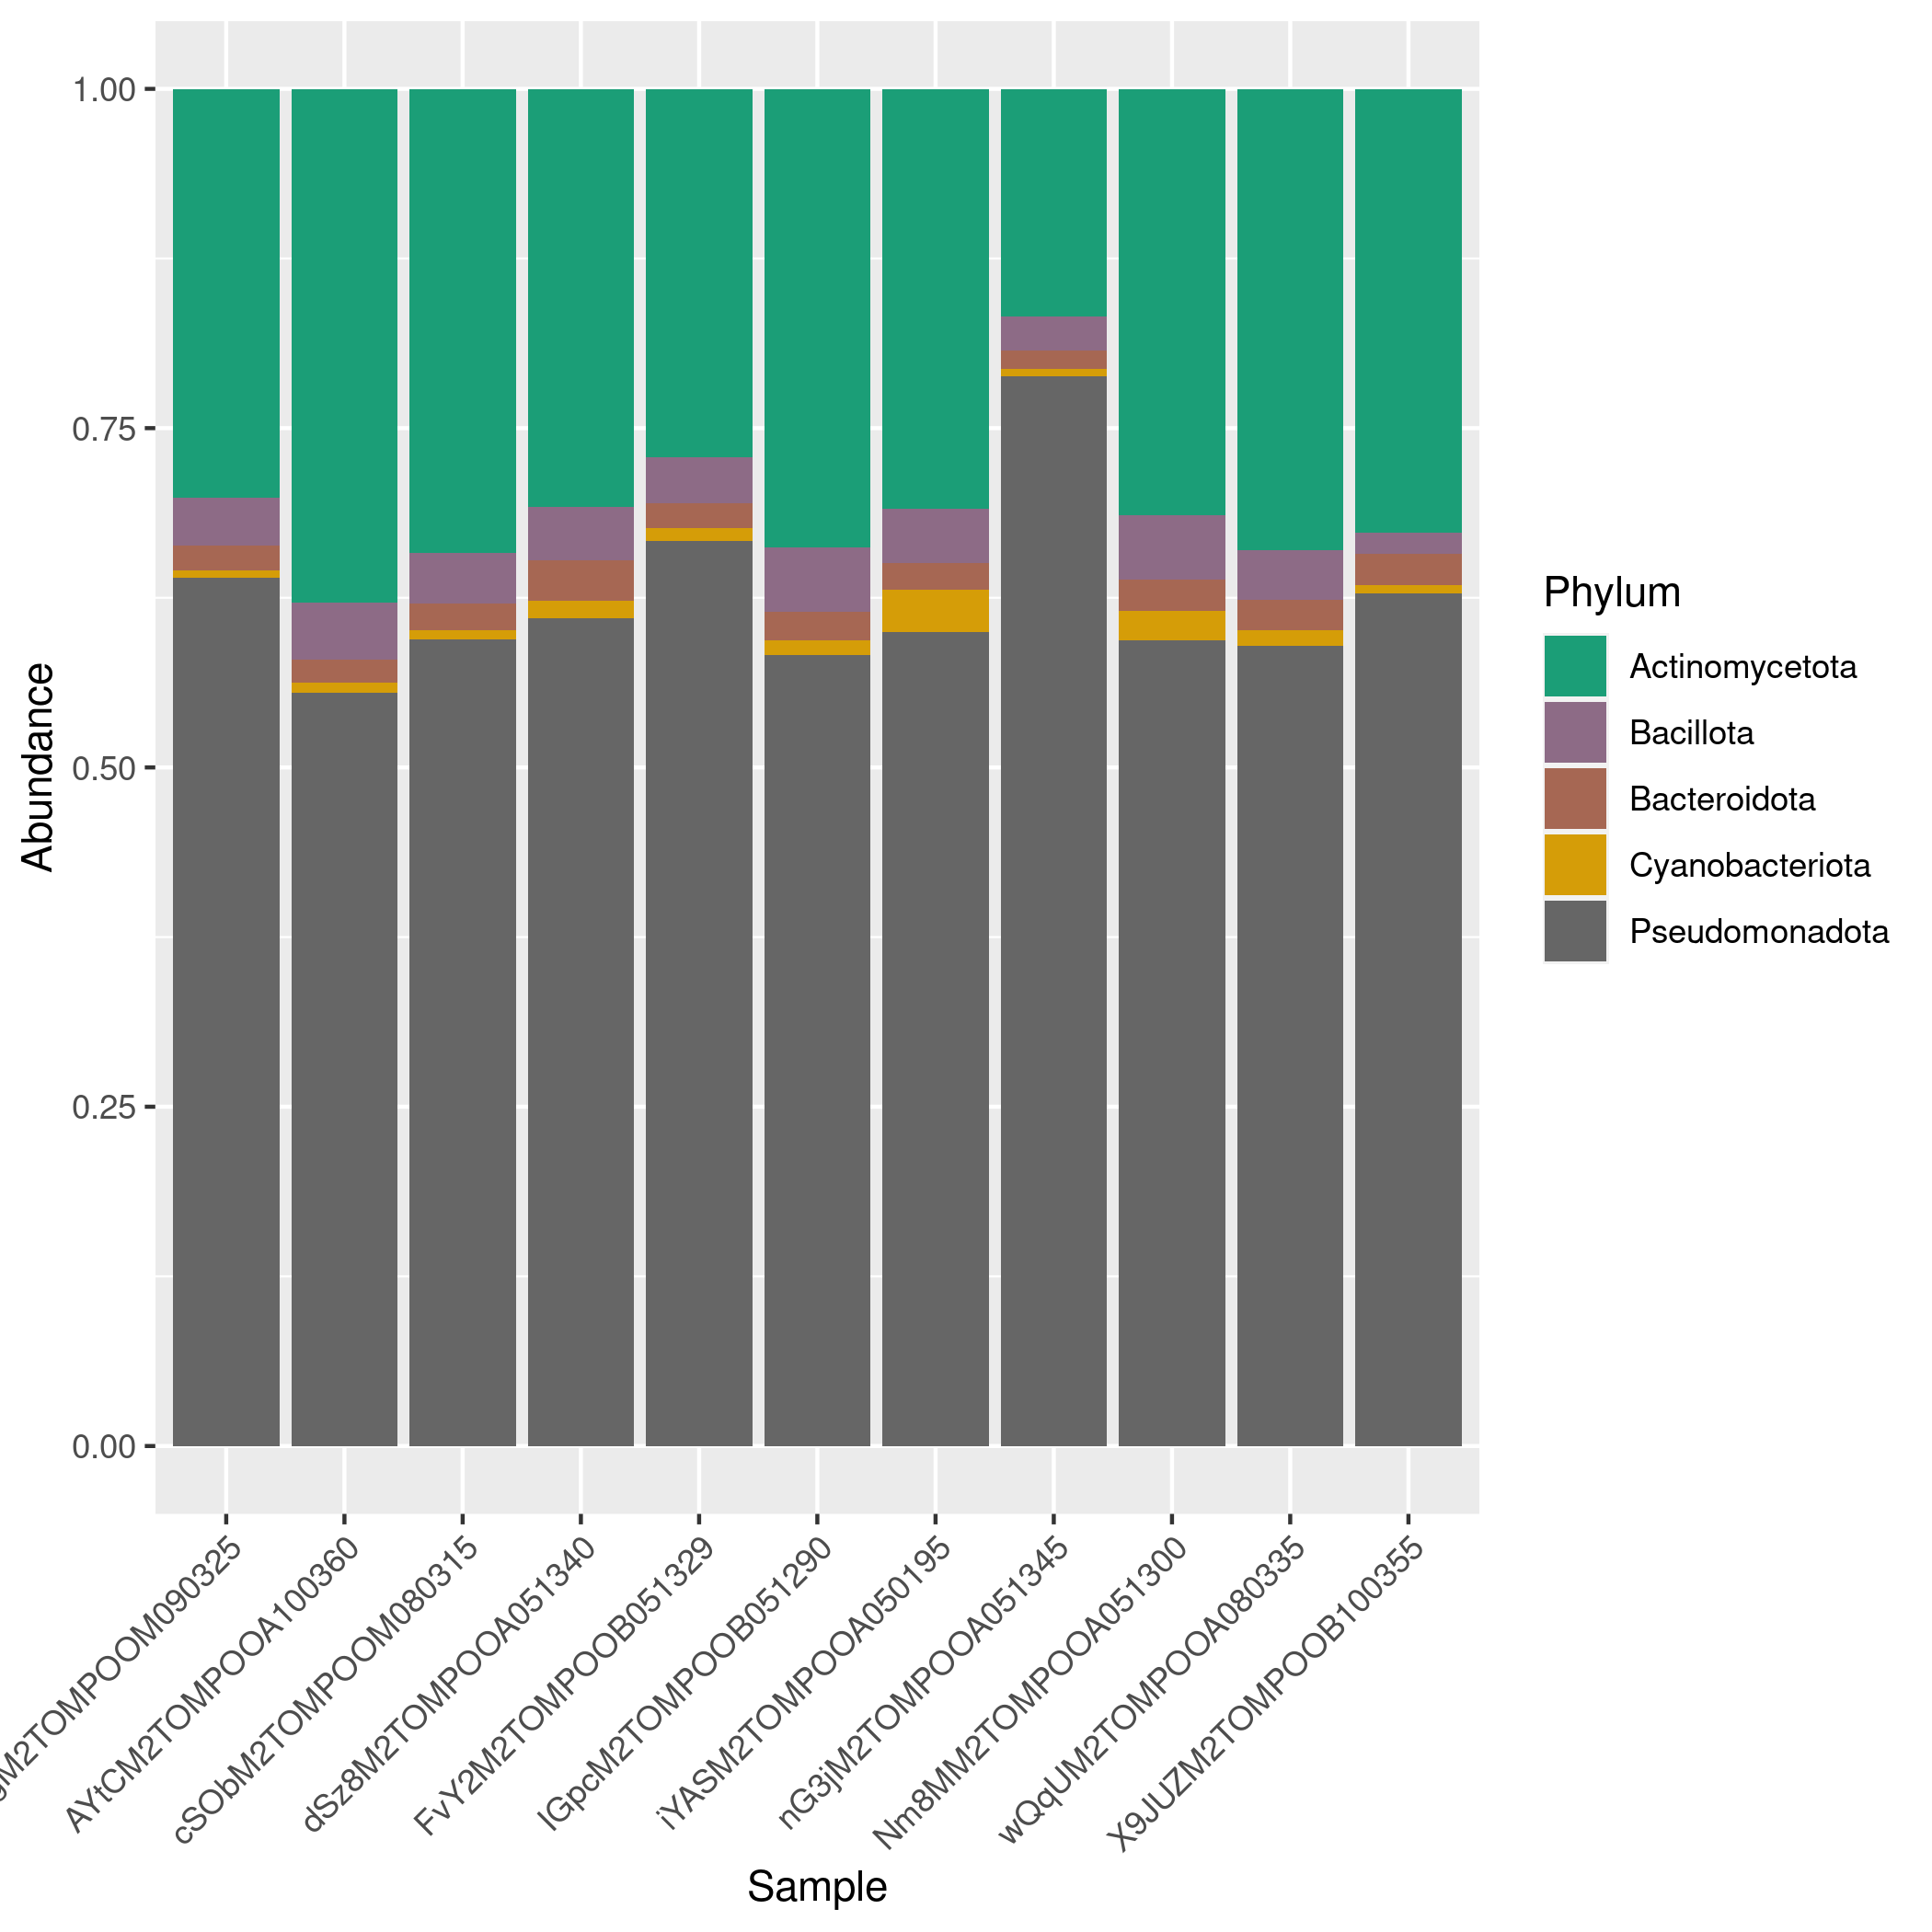
\includegraphics[scale = 0.8]{tomate_aleatorio1_5.csv_relative_abundance_Phylum.png}
\caption{Relative abundance by phyla of keystone OTUs }
\label{fig:tomate_aleatorio1_5.csv_phyla}
\end{figure}
\begin{figure}
\centering
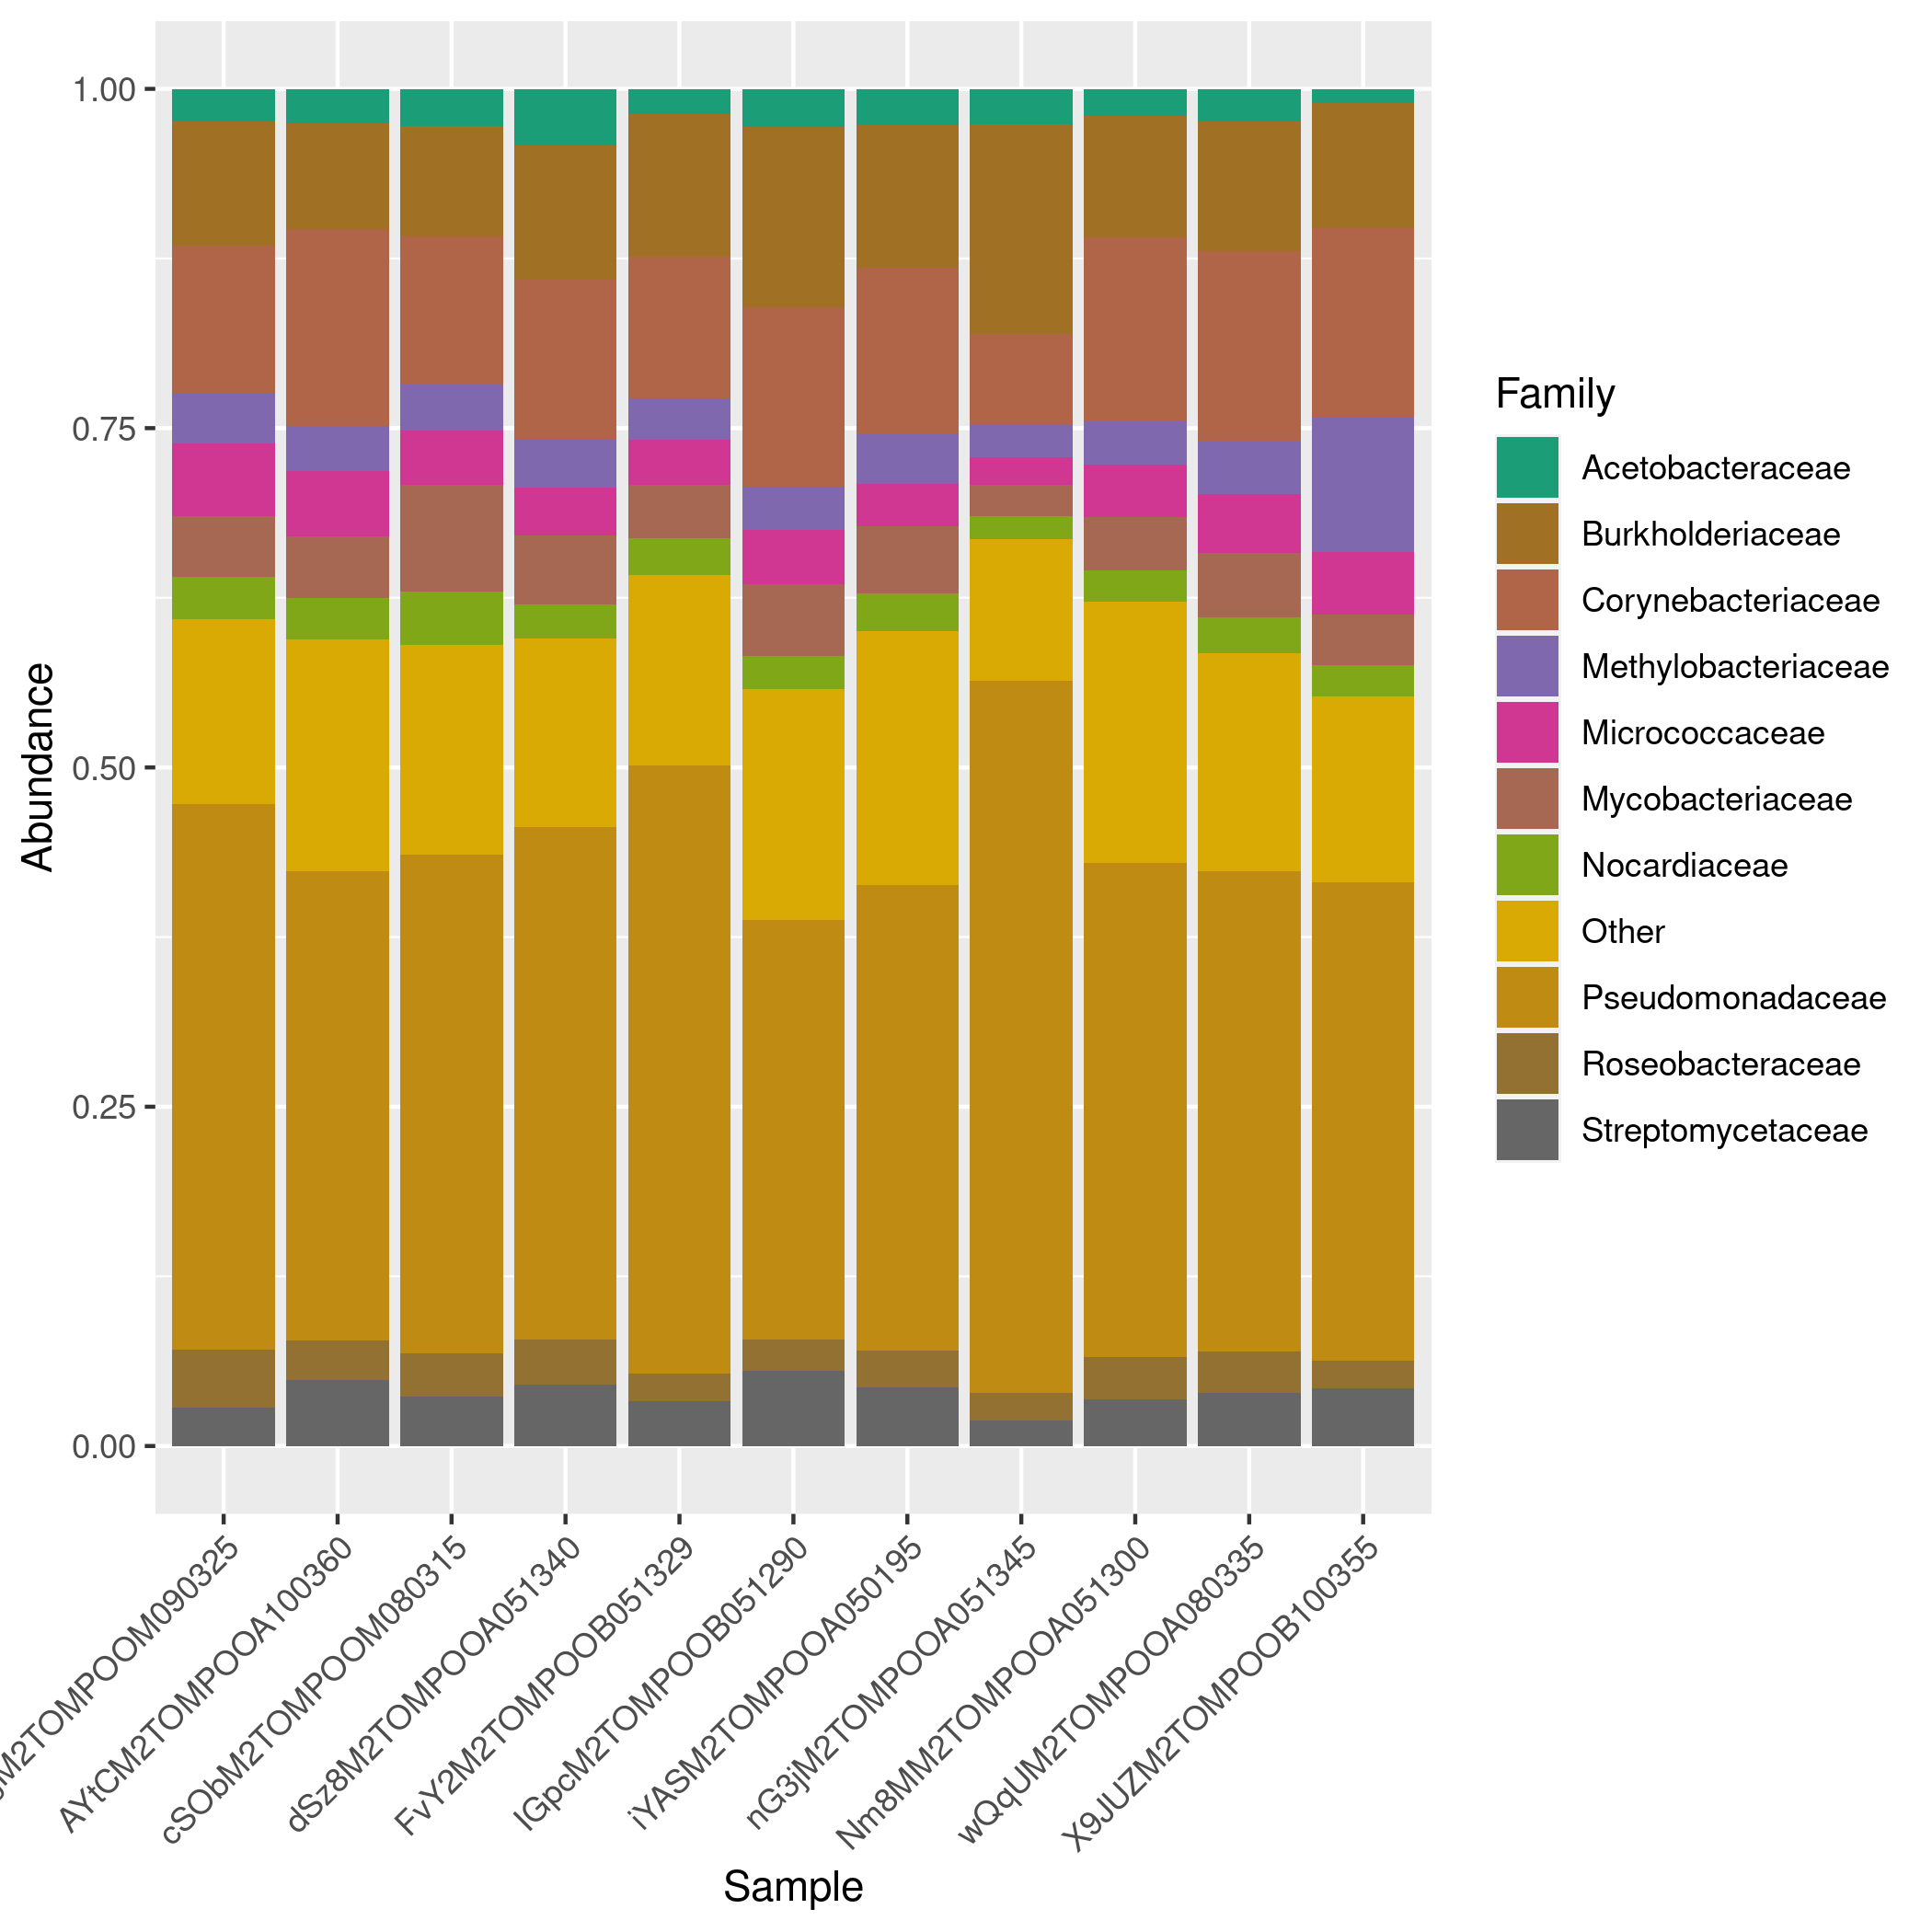
\includegraphics[scale = 0.8]{tomate_aleatorio1_5.csv_relative_abundance_Family.png}
\caption{Relative abundance by families of keystone OTUs }
\label{fig:tomate_aleatorio1_5.csv_family}
\end{figure}
\begin{figure}
\centering
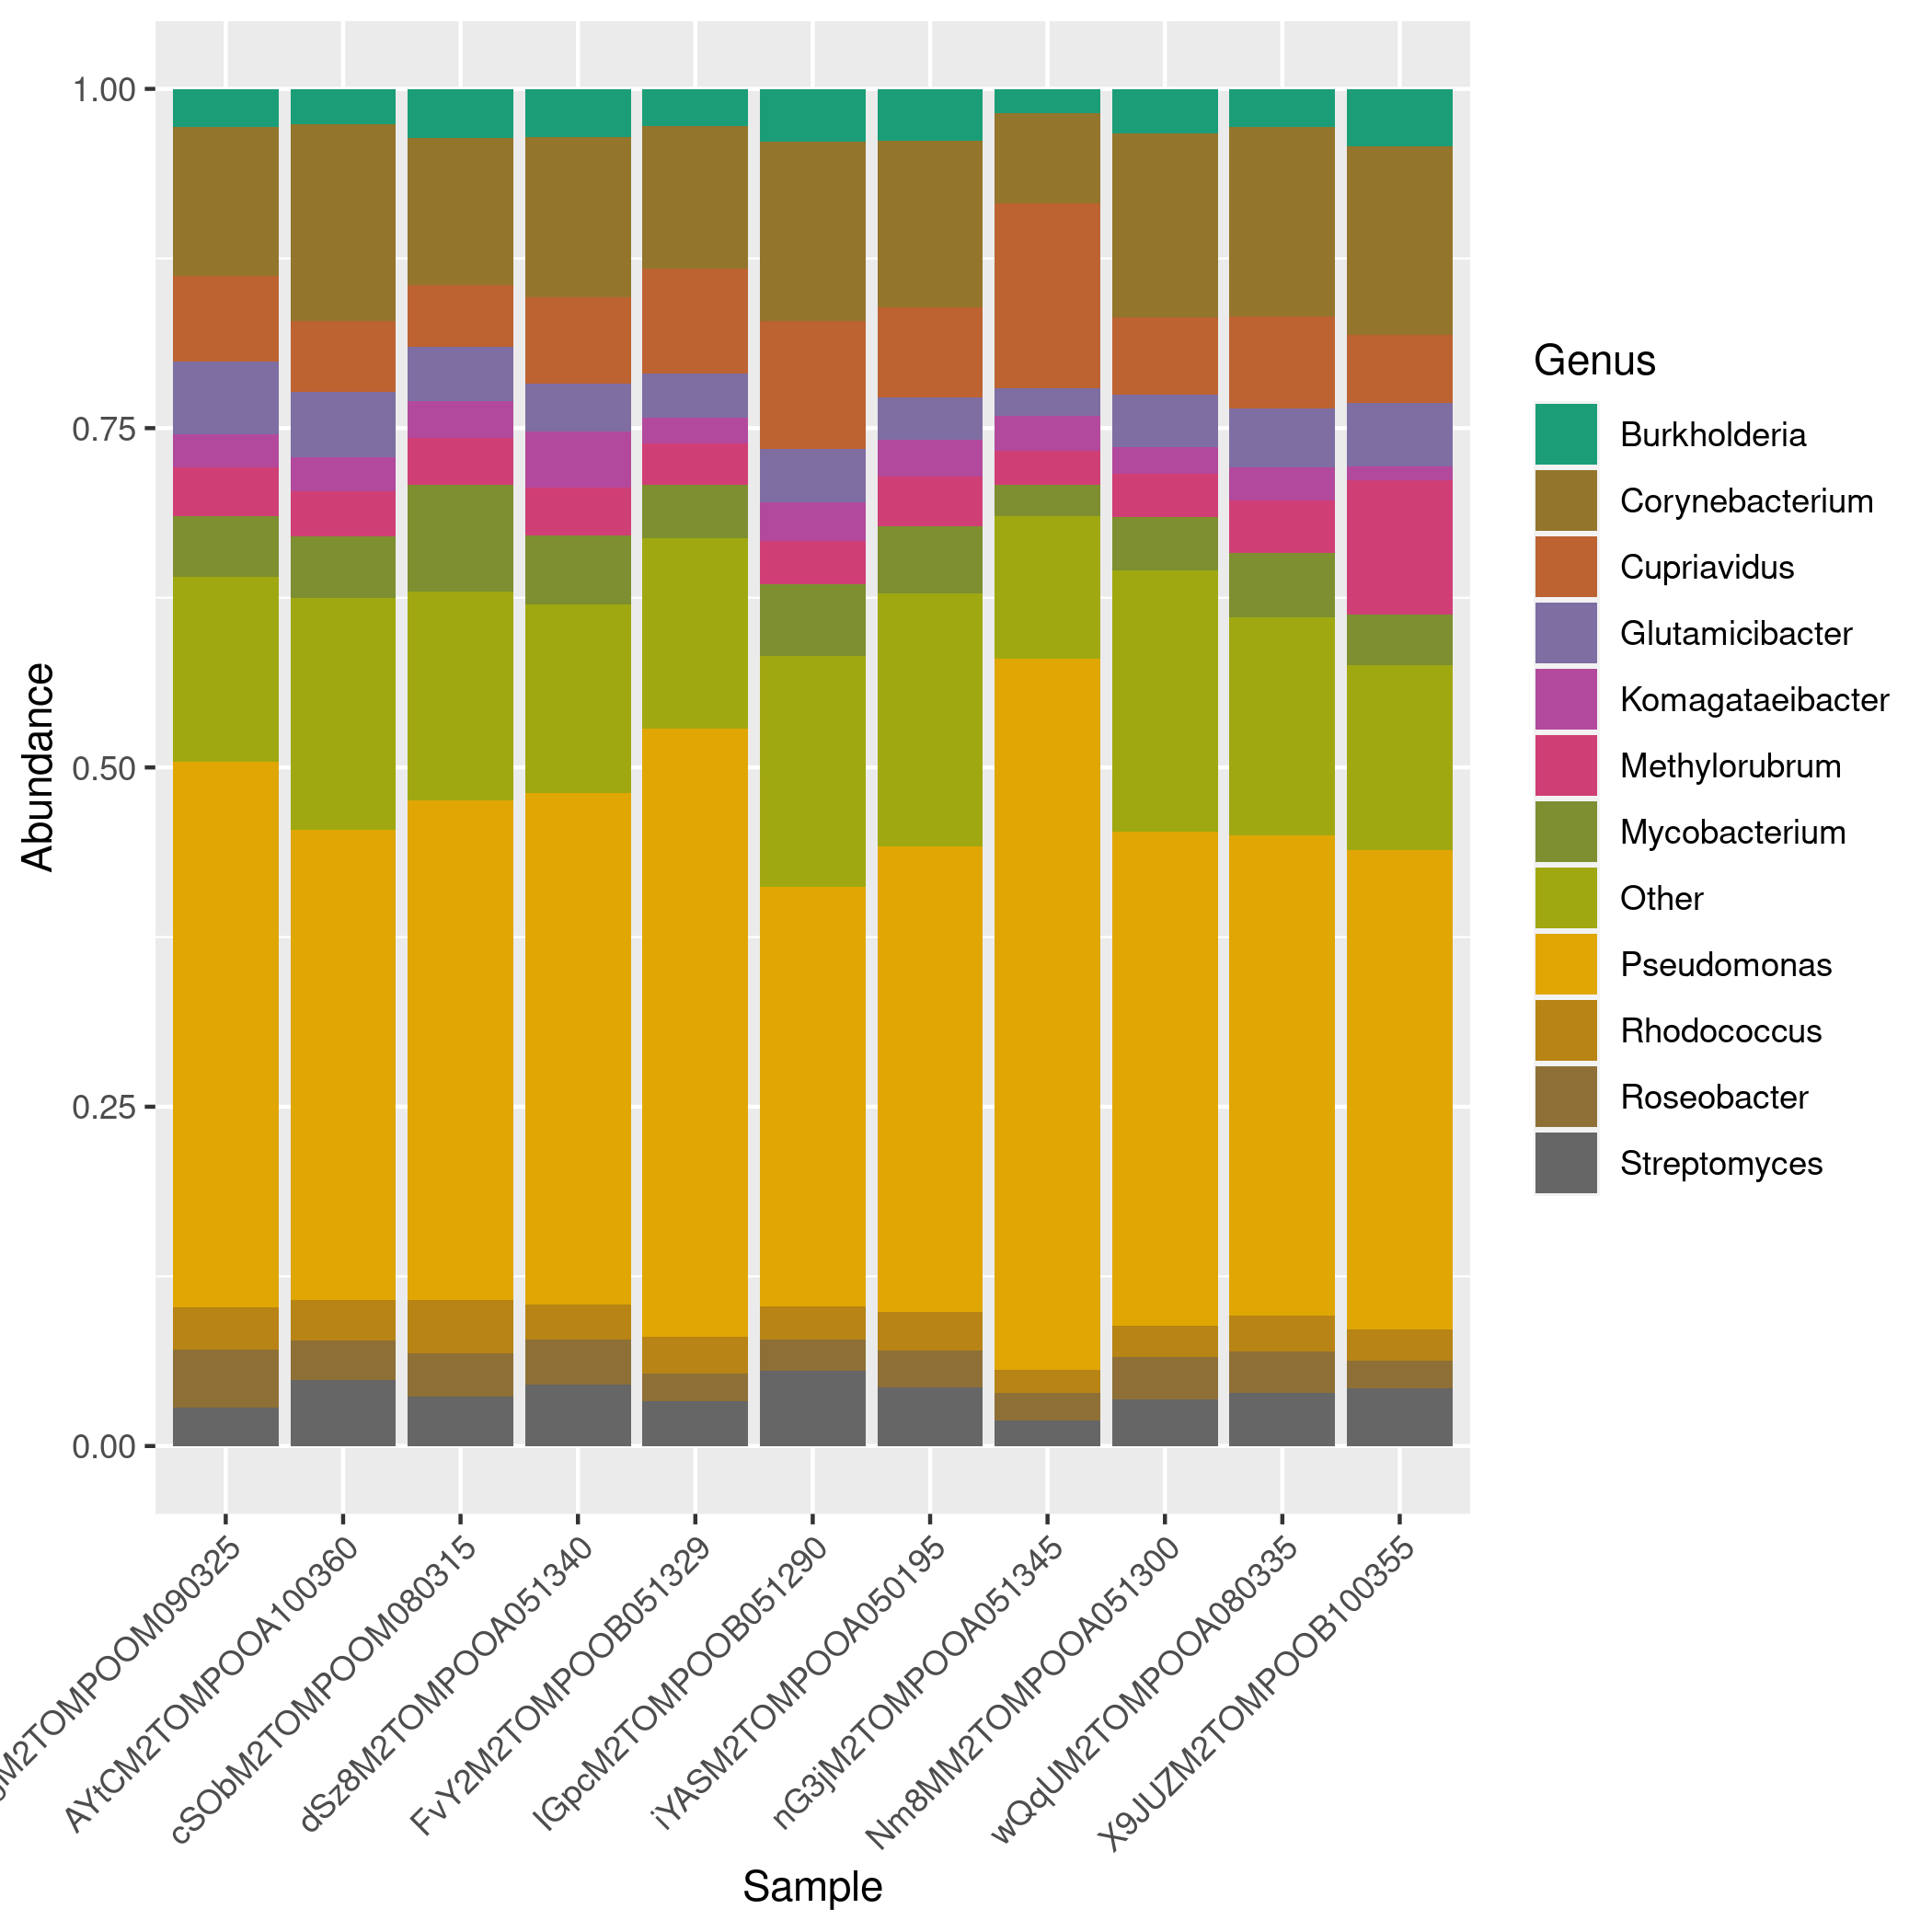
\includegraphics[scale = 0.8]{tomate_aleatorio1_5.csv_relative_abundance_Genus.png}
\caption{Relative abundance by genera of keystone OTUs }
\label{fig:tomate_aleatorio1_5.csv_genus}
\end{figure}
\begin{figure}
   \centering
   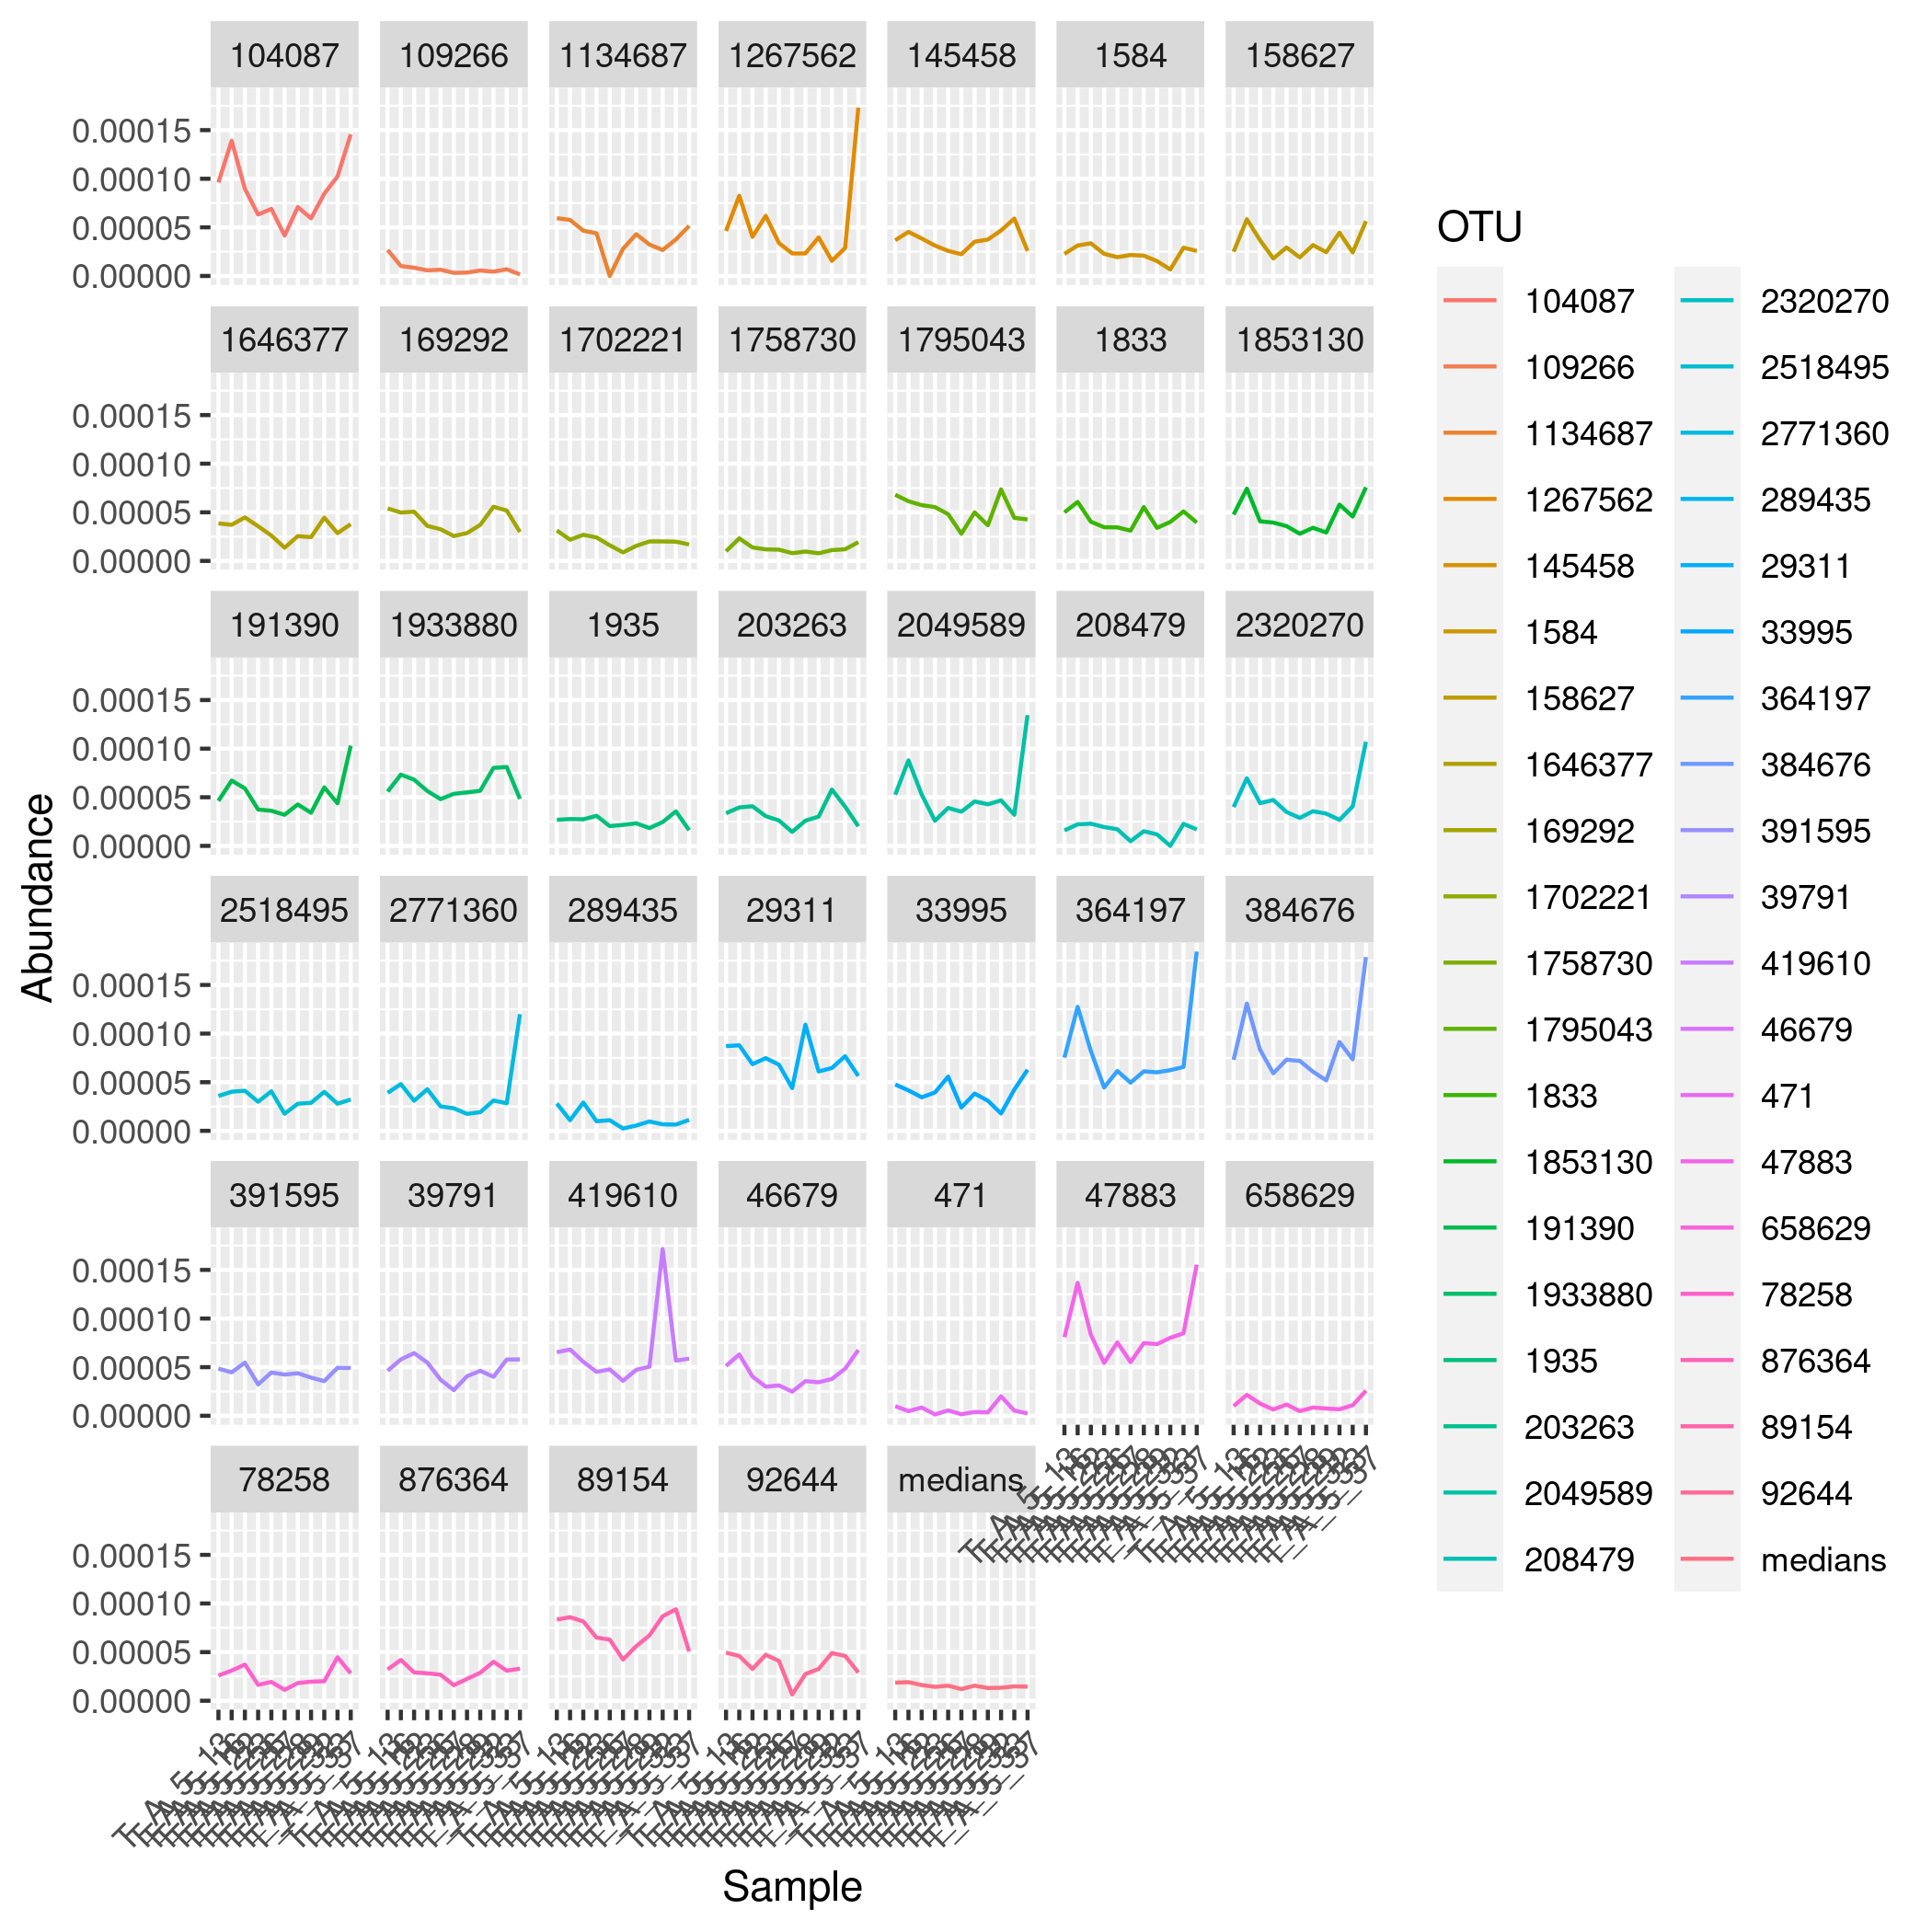
\includegraphics[scale = 0.8]{abundance_tomate_aleatorio1_5.csv_key_otus_medians.png}
   \caption{Plots representing relative abundance of each keystone OTU and one representing the median relative abundance  across samples of rhizosphere of tomate_aleatorio1_5.csv. Most keystone OTUs have relative abundance bigger than the median across all samples.  }
   \label{key_otus_vs_medians_tomate_aleatorio1_5.csv}
\end{figure}
\begin{figure}
 \centering
 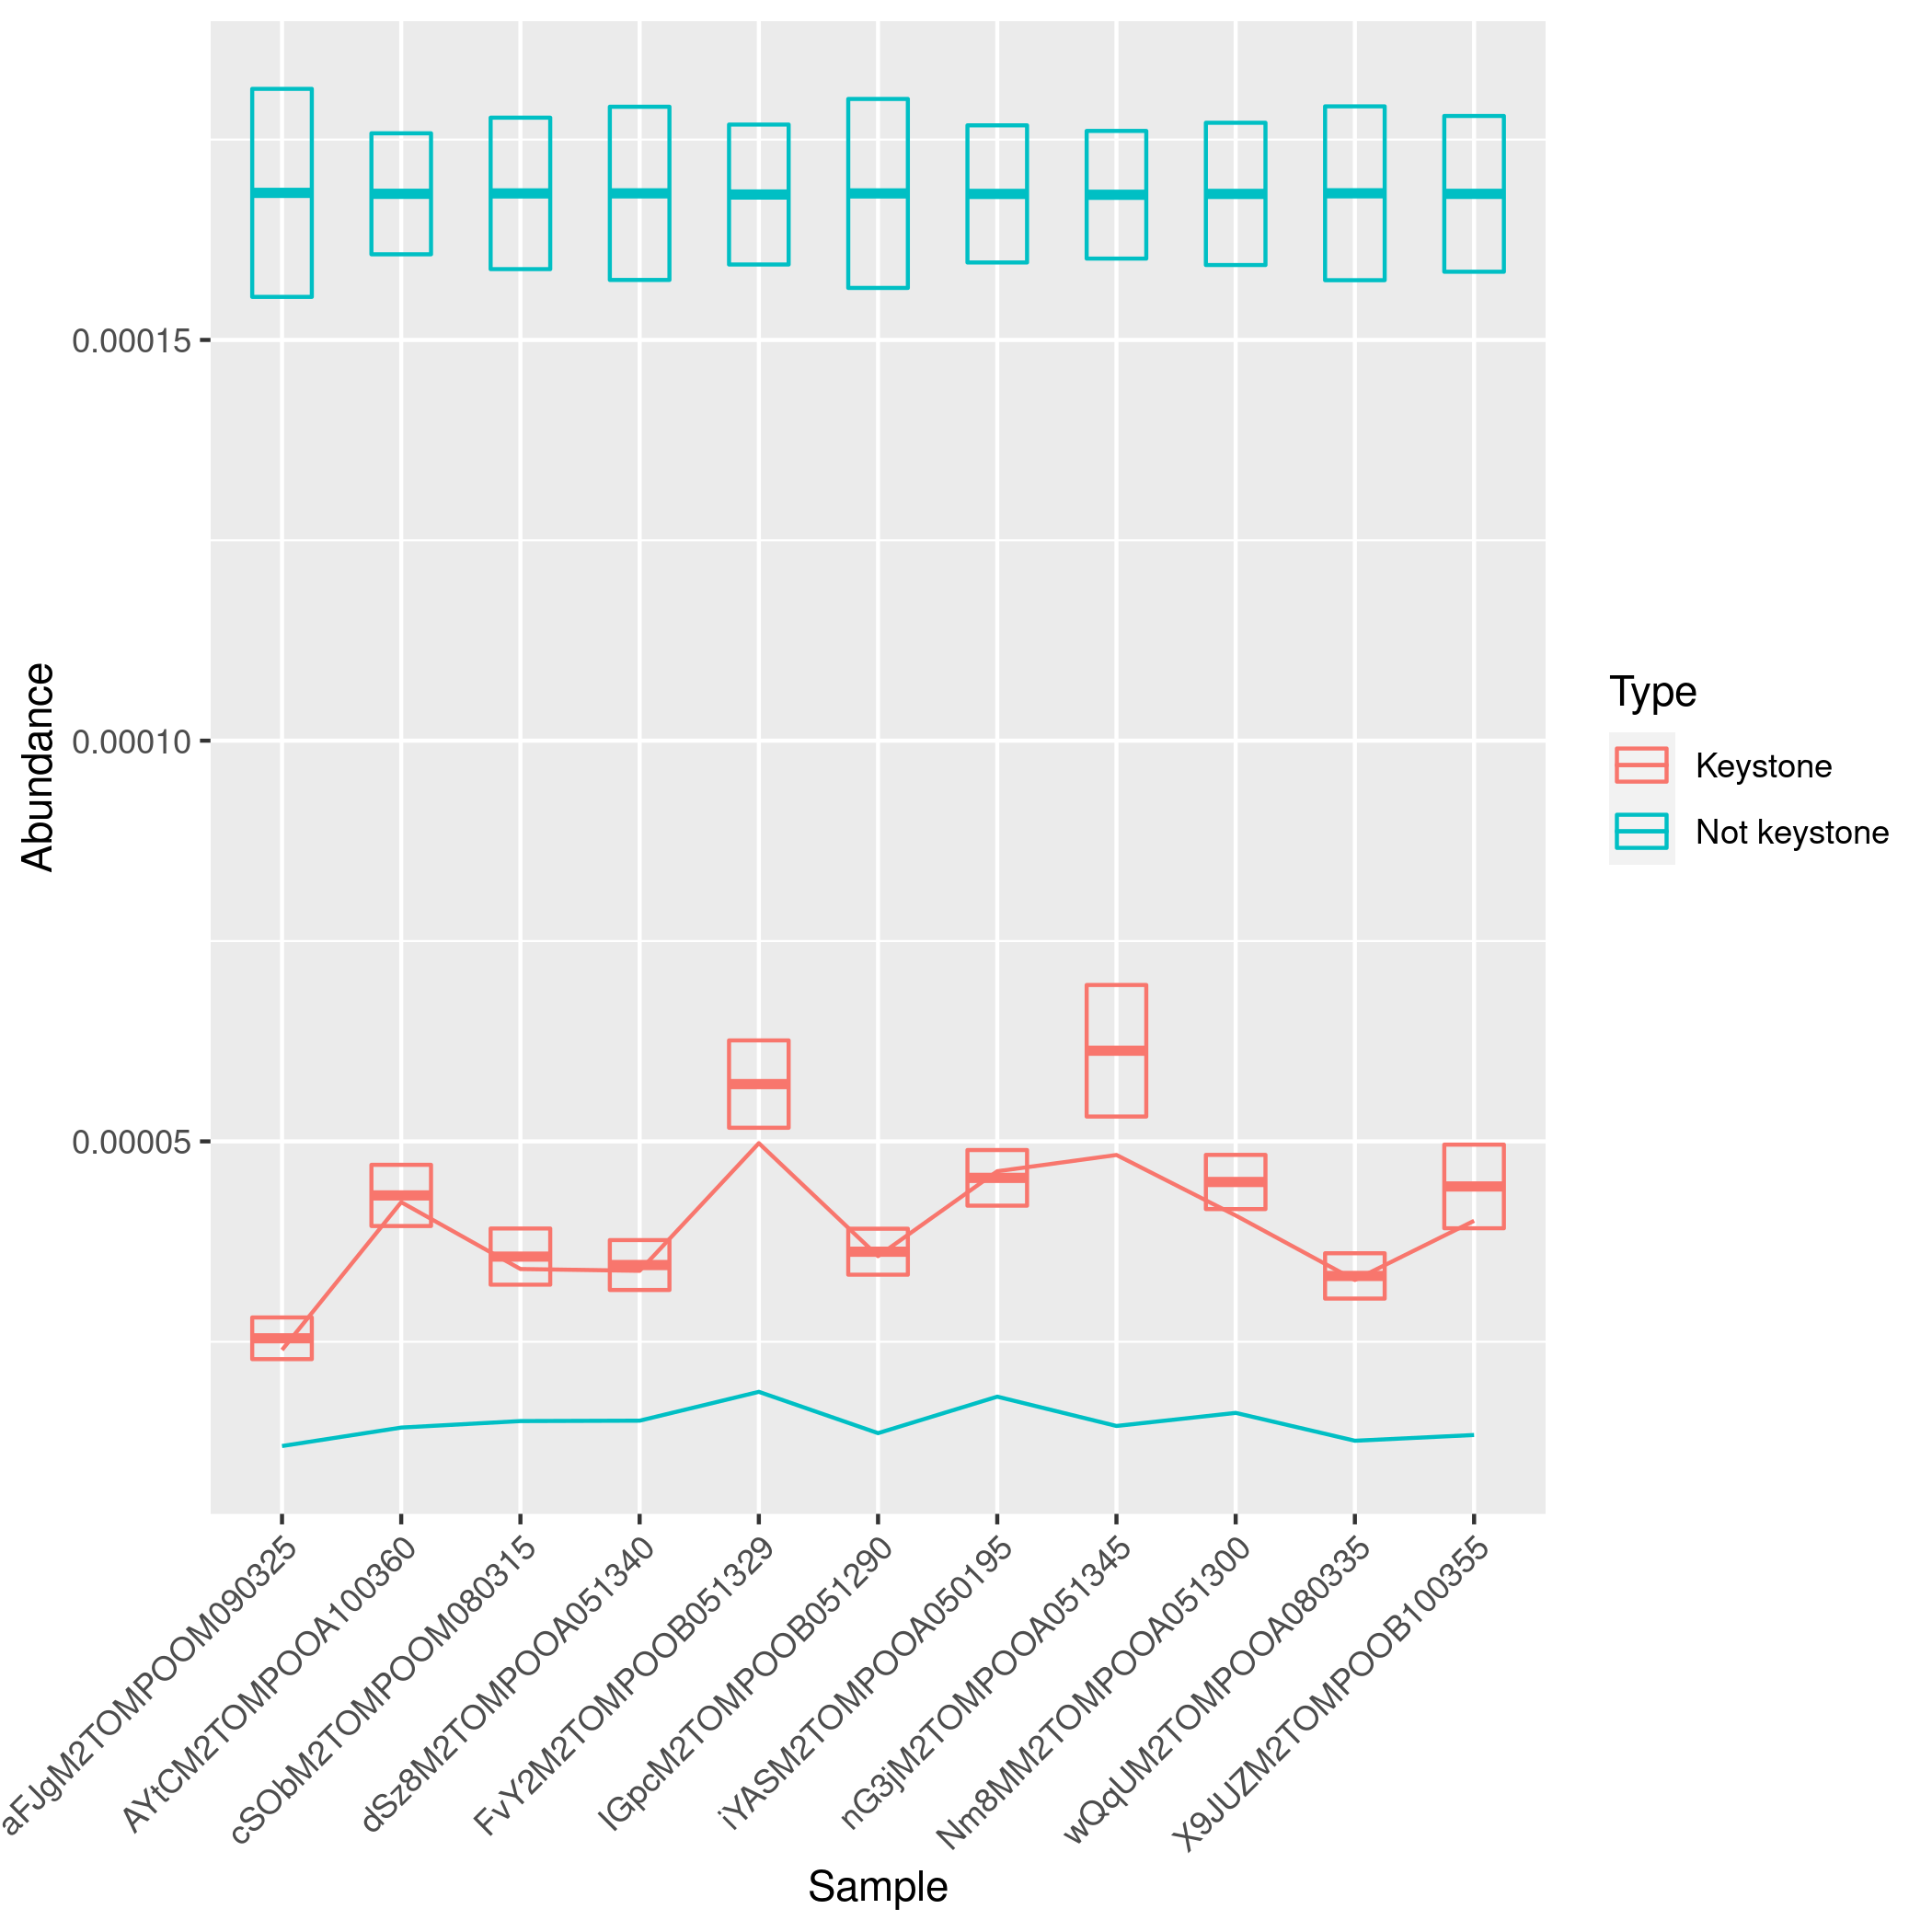
\includegraphics[scale = 0.75]{mean_median_key_vs_not_key_tomate_aleatorio1_5.csv.png}
\caption{Boxes represent mean and standard error in the distribution of corresponding samples. Lines represent the corresponding medians. In these samples of rhizosphere oftomate_aleatorio1_5.csv}
\label{mean_median_tomate_aleatorio1_5.csv}
\end{figure}
\begin{figure}
   \centering
   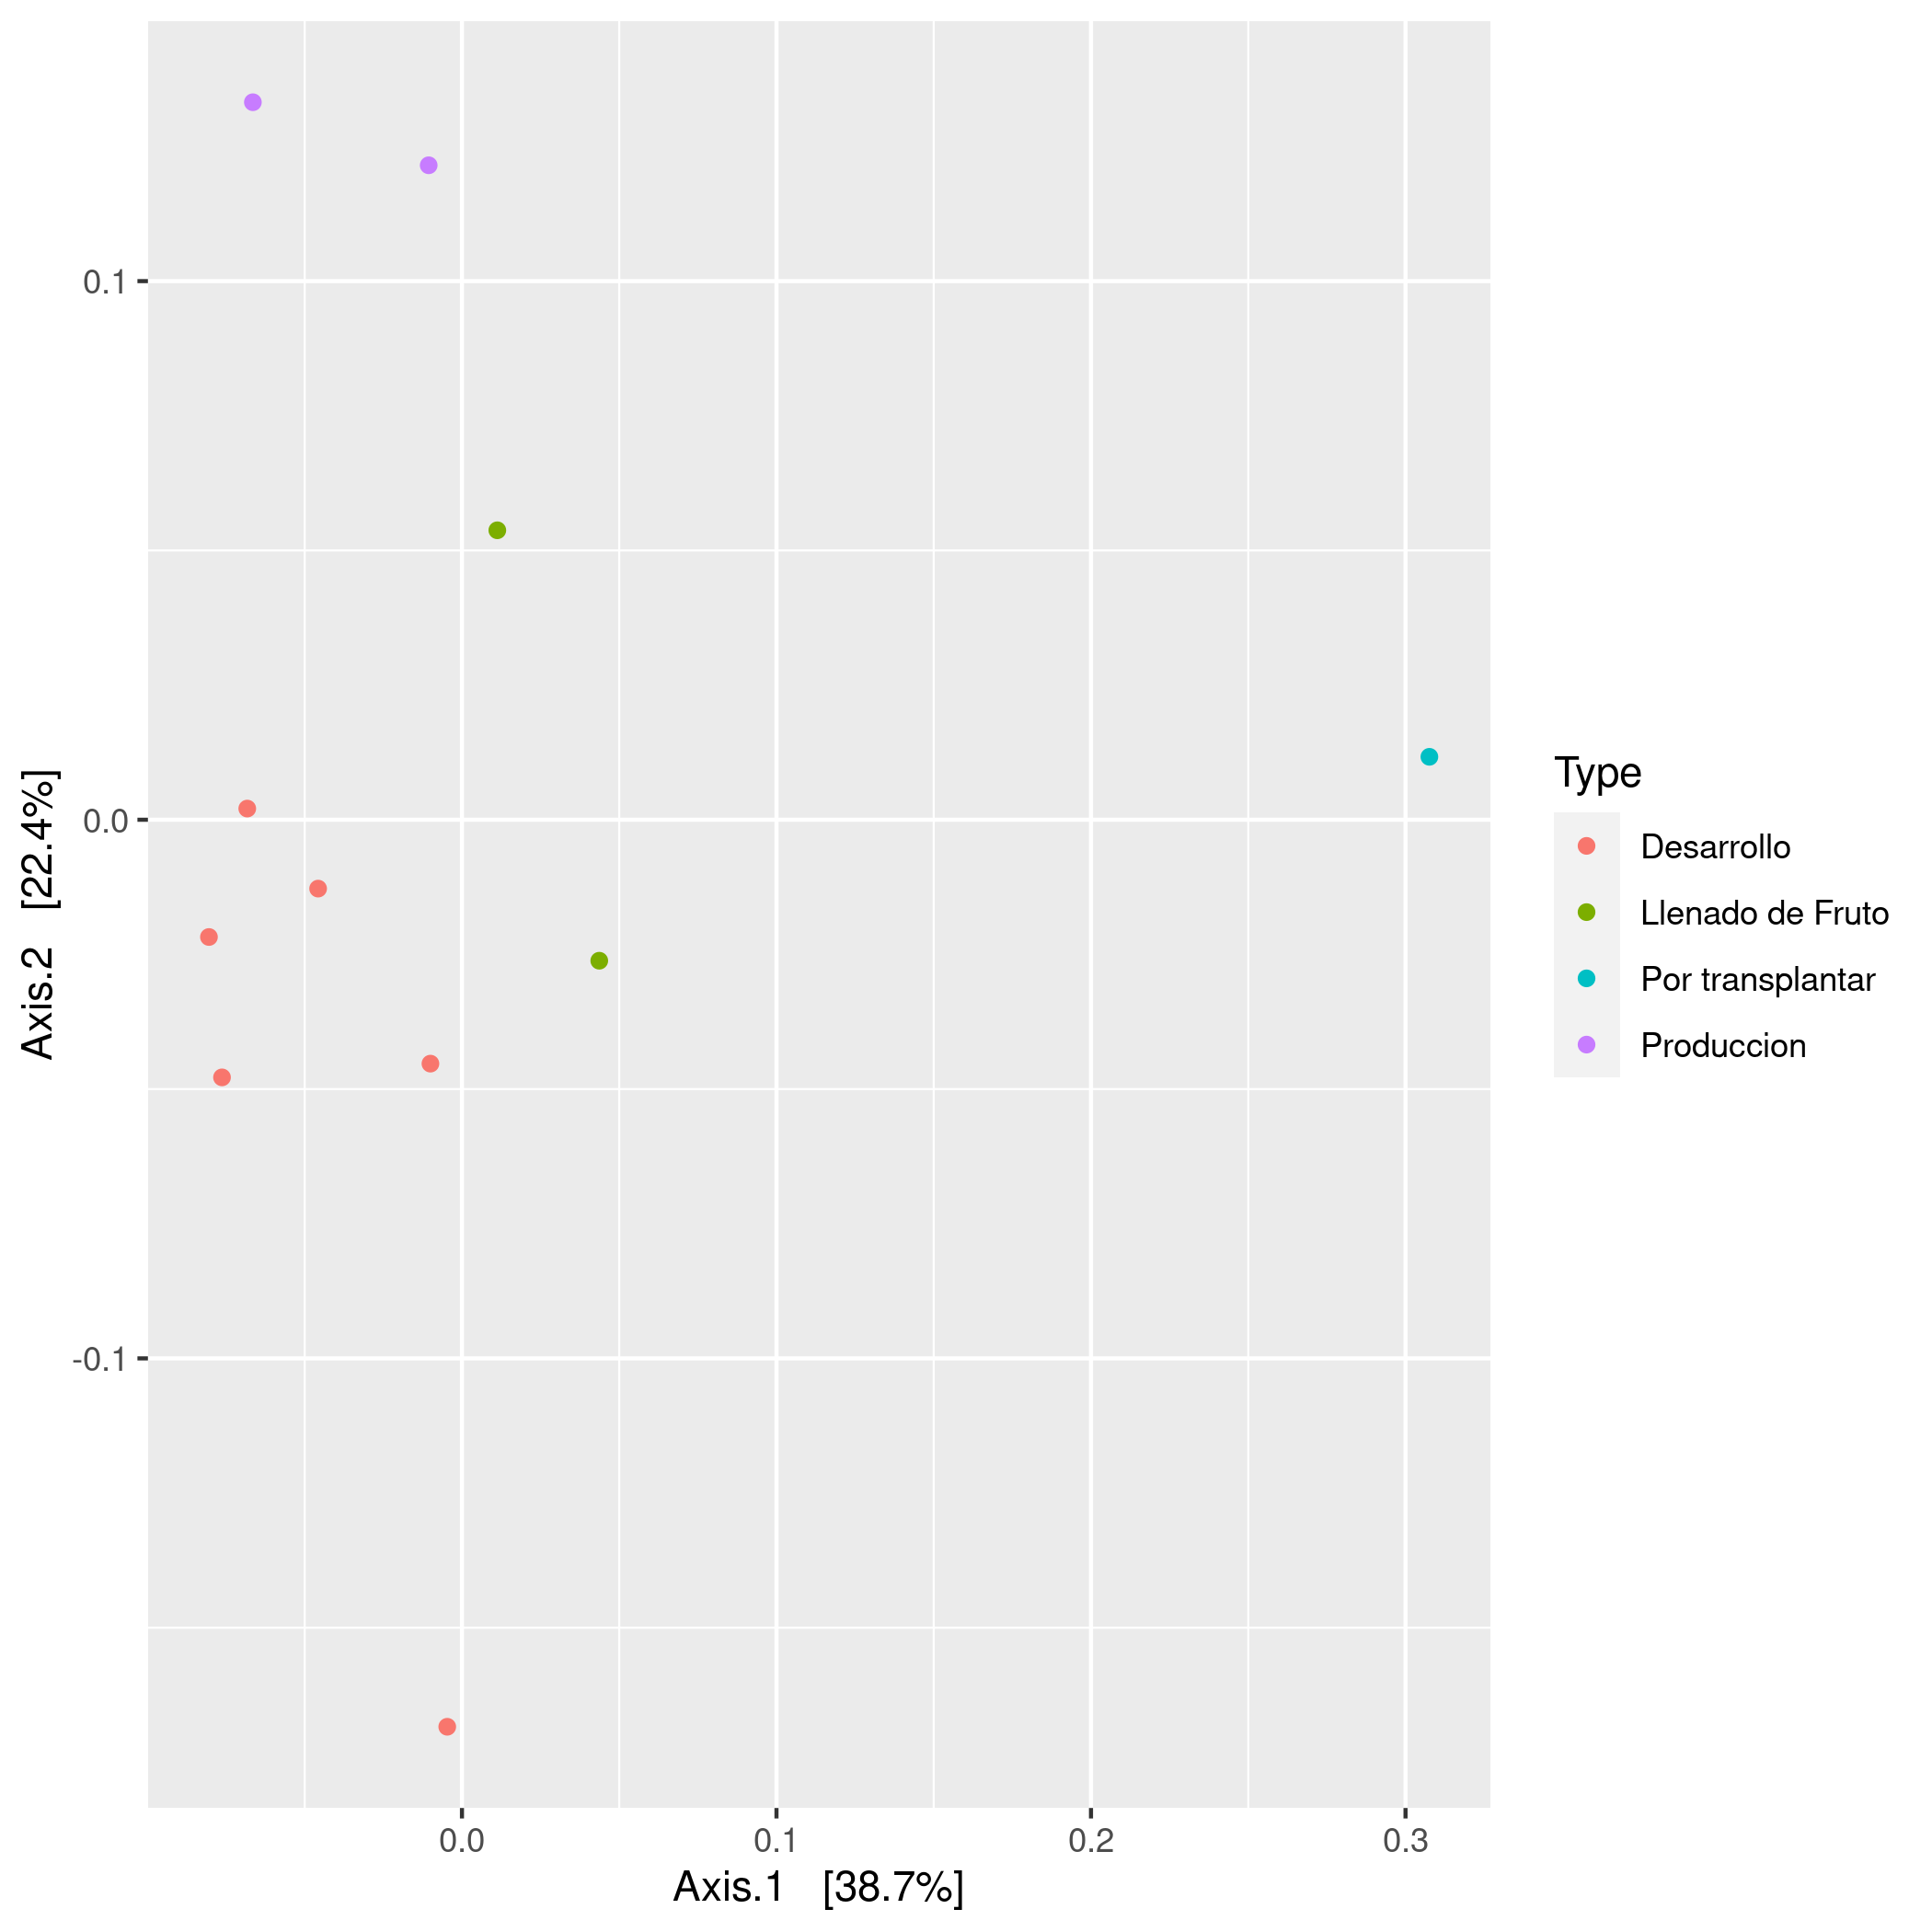
\includegraphics[scale = 0.7]{pcoa_muestras_tomate_aleatorio1_5.csv.png}
 \caption{PCoA analysis with Bray-Curtis distance of rhizosphere samples of tomate_aleatorio1_5.csv.}
 \label{fig:tomate_aleatorio1_5.csv_pcoa}
\end{figure}
\begin{figure}
  \centering
  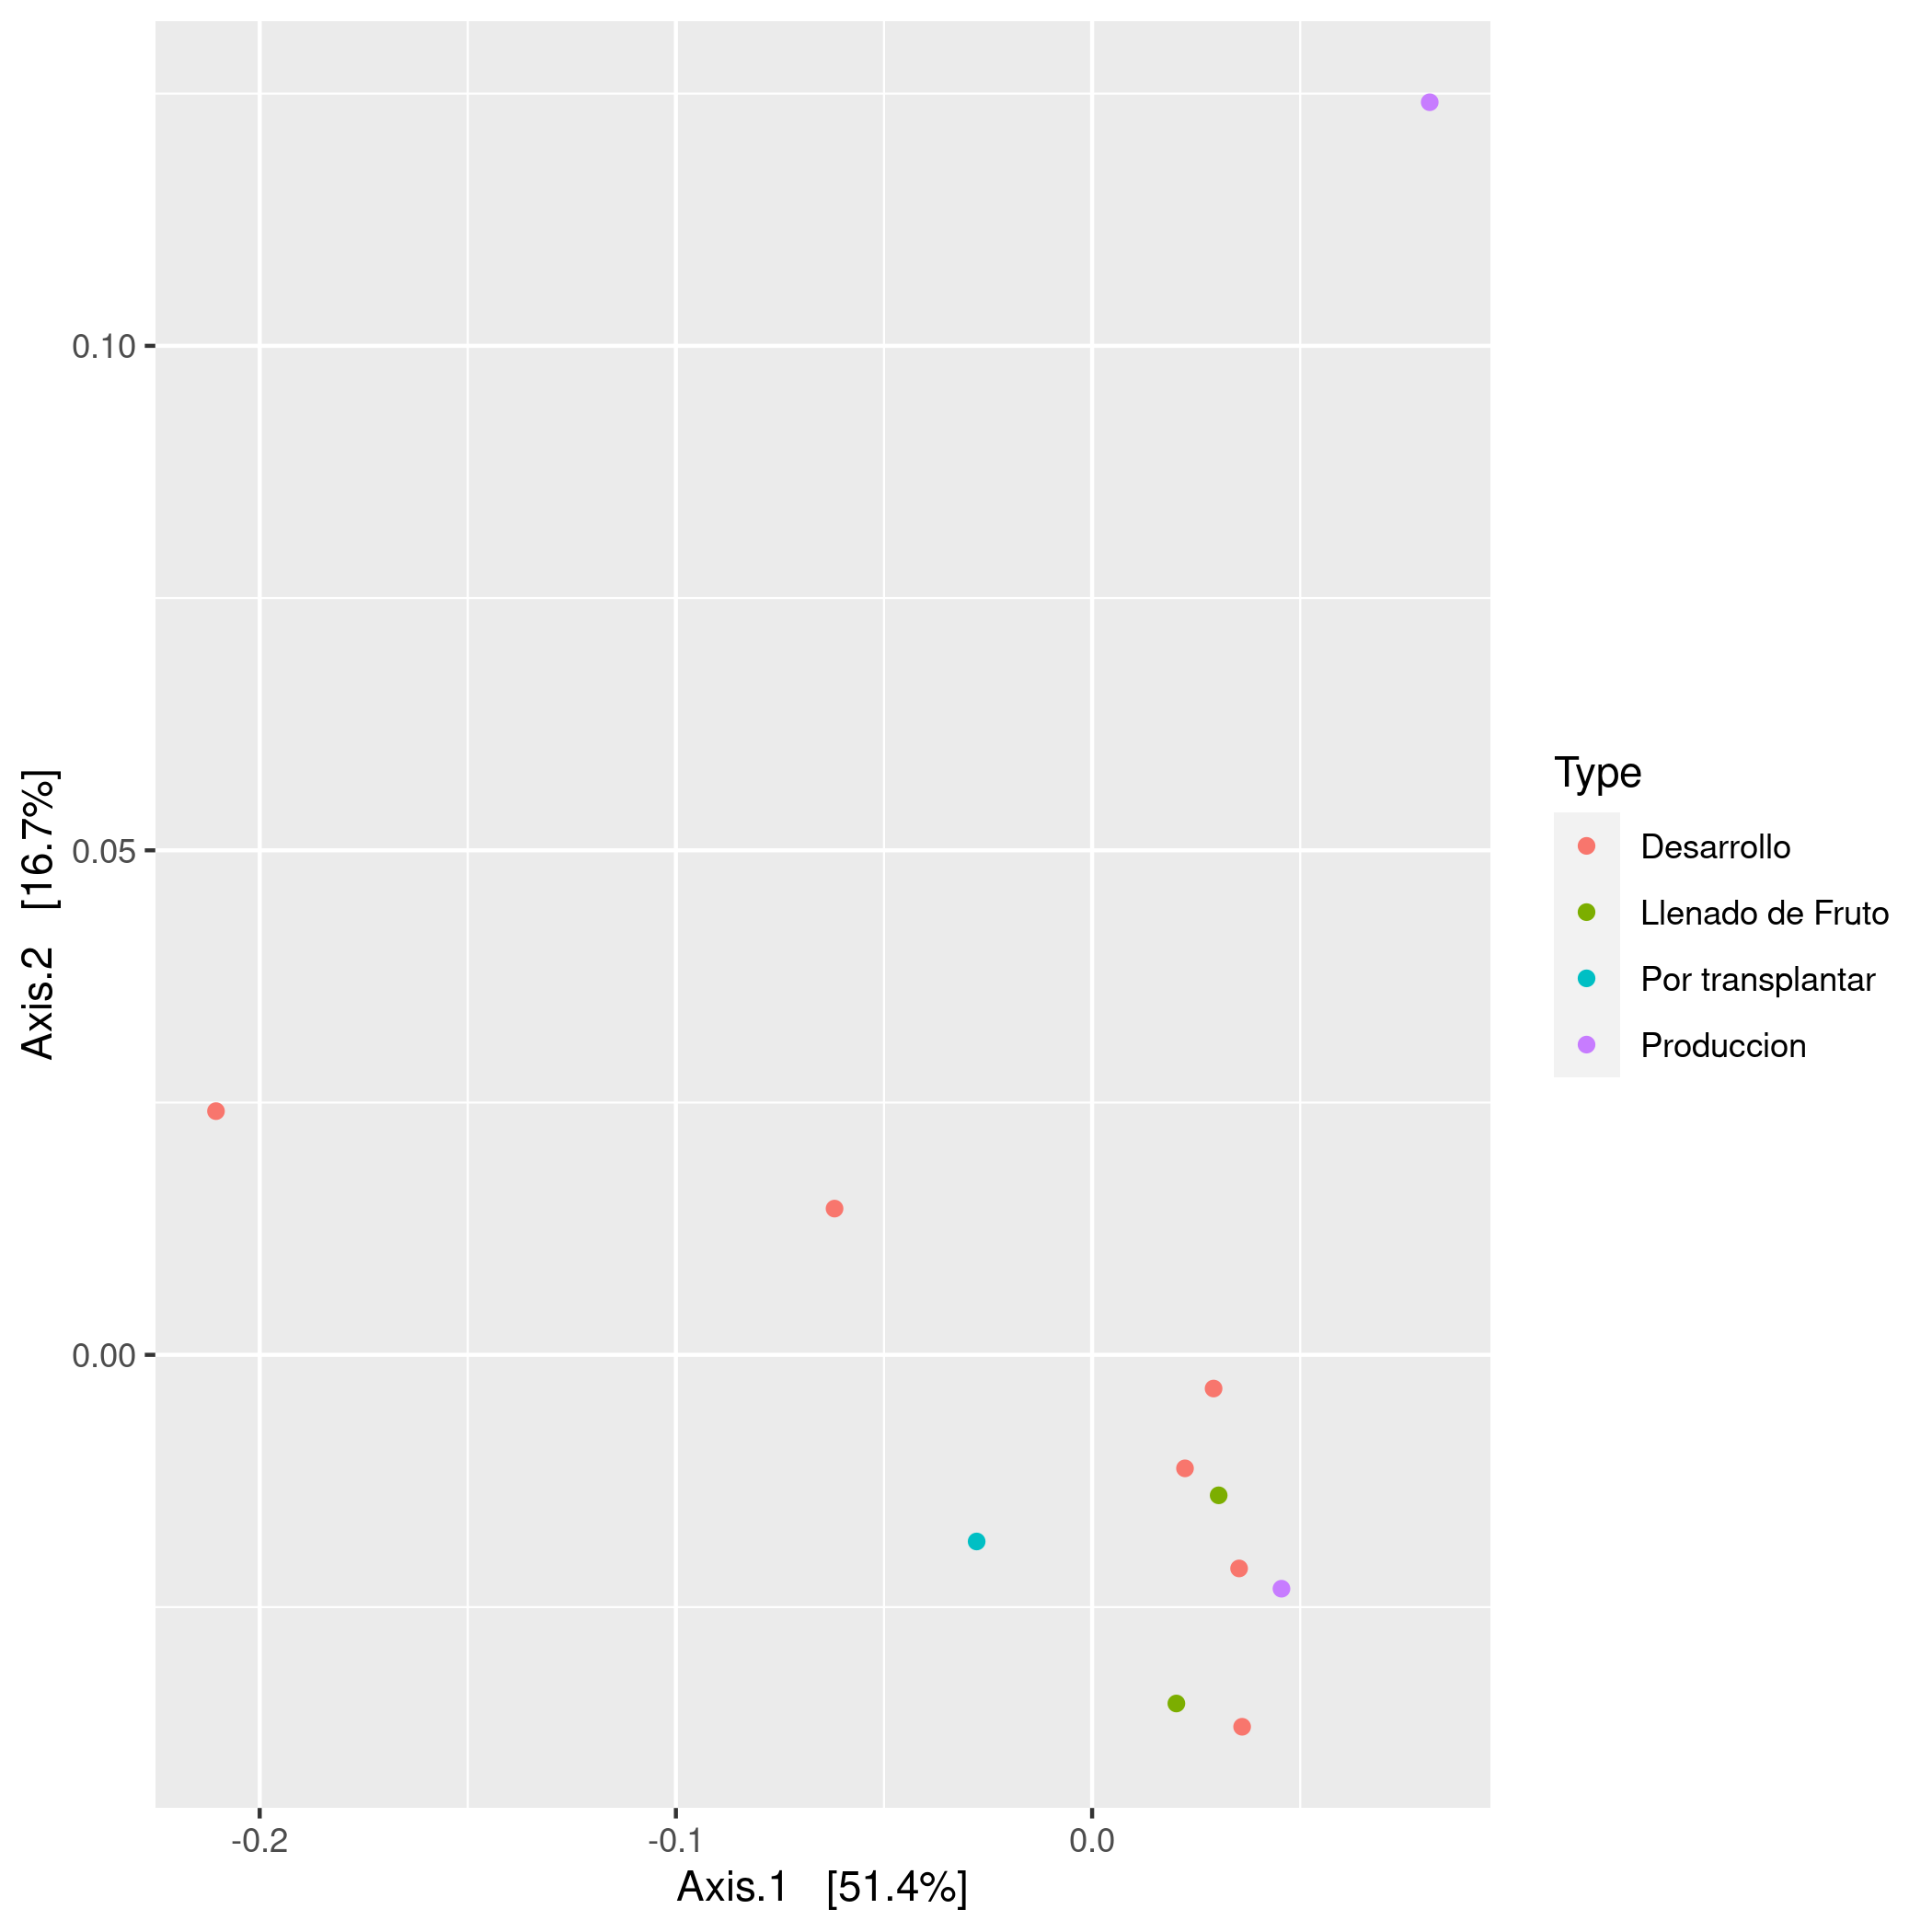
\includegraphics[scale = 0.7]{pcoa_key_otus_tomate_aleatorio1_5.csv.png}
  \caption{PCoA analysis with Bray-Curtis distance of rhizosphere samples of tomate_aleatorio1_5.csv, restricted to keystone OTUs.}
  \label{fig:tomate_aleatorio1_5.csv_pcoa_key_otus}
\end{figure}
